\begin{appendices}

%Some Table of Contents entry formatting
\addtocontents{toc}{\protect\renewcommand{\protect\cftchappresnum}{\appendixname\space}}
\addtocontents{toc}{\protect\renewcommand{\protect\cftchapnumwidth}{6em}}

%Begin individual appendices, separated as chapters

\chapter[\texorpdfstring{Linklet Kernel Language Specification}{Appendix A}]{Linklet Kernel Language Specification}
\label{appendix:linklet-kernel-language}

    \inputAppendixFigure{linklet-kernel-language-grammar.tex}

    \begin{figure}[h]
    \centering
    \fbox{
        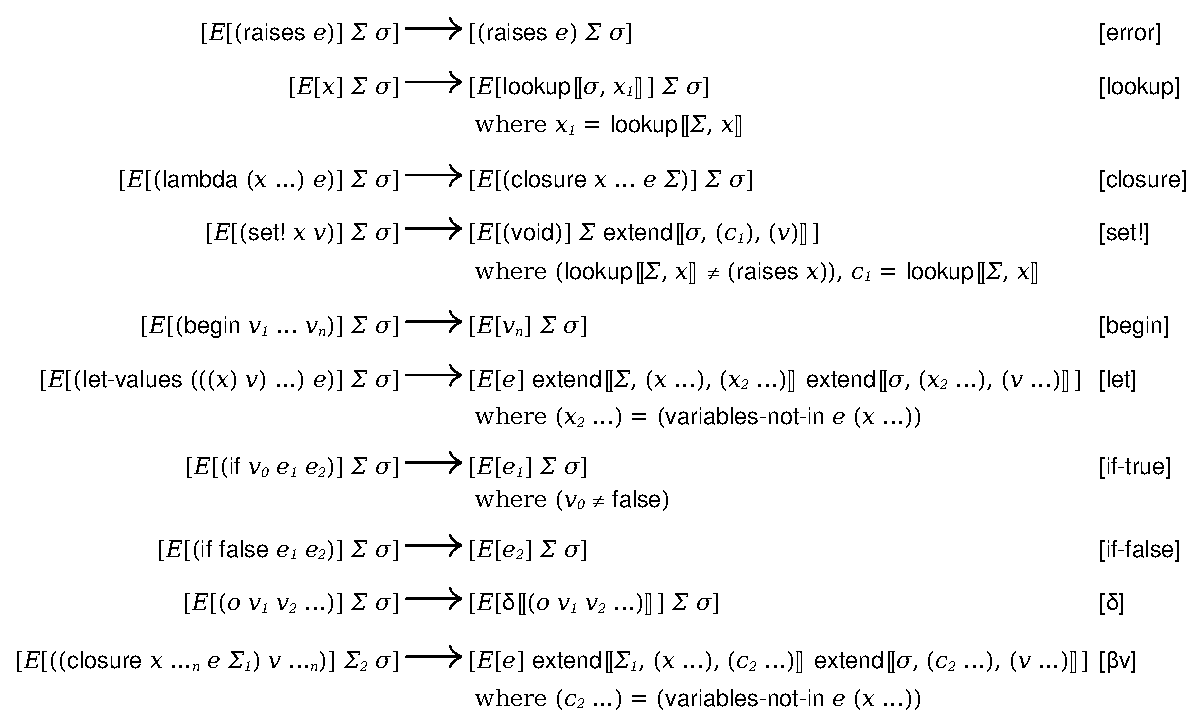
\includegraphics[scale=0.8]{sections/figures/rc-red-relation.eps}
    }
    \caption{Linklet Kernel Language standard reduction relation}
    \label{fig:rc-red-relation}
    \end{figure}

    \begin{figure}[h]
    \centering
    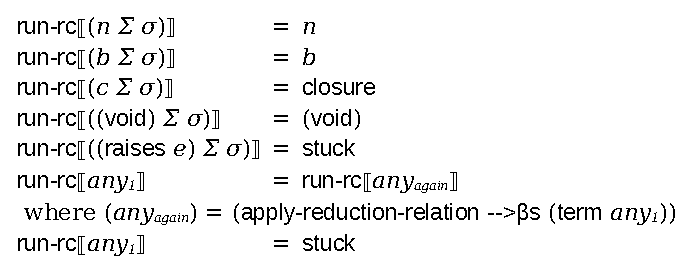
\includegraphics[scale=1]{sections/figures/rc-run-rc.eps}
    \caption{Linklet Kernel Language evaluator}
    \label{fig:rc-run-rc}
    \end{figure}


\chapter[\texorpdfstring{Complete Reduction Steps for Top-level Example Program}{Appendix B}]{Complete Reduction Steps for Top-level Example Program}
\label{appendix:formal-reduction-steps-toplevel-example}

    \inputAppendixFigure{complete-toplevel-example-step-by-step-formal.tex}

\chapter[\texorpdfstring{PLT Redex Model for Linklet Semantics}{Appendix C}]{PLT Redex Model for Linklet Semantics}
\label{appendix:linklet-semantics-model-redex-code}

    \inputAppendixFigure{linklet-semantics-plt-redex-model.tex}

\chapter[\texorpdfstring{Semantics for the CEK \& Stackful Hybrid Model}
                          {Appendix D}]{Semantics for the CEK \& Stackful Hybrid Model}
\label{appendix:cek-stackful-redex}

    % \begin{figure}[!h]
% \centering
% \footnotesize
% %--- tweak the padding between text and frame (optional) ---
% \setlength{\fboxsep}{6pt}% default is 3 pt
% %--- boxed grammar -----------------------------------------
% \fbox{%
%     \begin{minipage}{0.5\linewidth}
%     \begin{align*}
%         e &::=\; x\; |\; v\; |\; (e\; e\; \ldots)\; |\; (\textbf{if}\; e\; e\; e)\; |\; (o\; e\; e)\; \\
%         &\; |\; (\textbf{begin}\; e\; e\; \ldots)\; |\; (\textbf{lambda}\; (x_{\_!\_}\; \ldots)\; e)\\
%         &\; |\; (\textbf{set!}\; x\; e)\; |\; (\textbf{raises}\; e)\\
%         &\; |\; (\textbf{let\dash values}\; (((x)\; e)\; \ldots)\; e)\\
%         &\; |\; (\textbf{convert\dash to\dash stackful}\; e)\\
%         &\; |\; (\textbf{convert\dash to\dash cek}\; e)
%     \end{align*}

%     \vspace{0.01em}

%     \end{minipage}}
% %-----------------------------------------------------------
% \caption[hede]{Source Language for Stackful \& CEK Models}
% \label{fig:st-cek-grammar}
% \end{figure}


\begin{figure}[!h]
\centering
\includegraphics[scale=1]{\inputFigPath{solution}{cek-stackful-grammar}}
\caption{Source Language for Stackful \& CEK Model [PLACEHOLDER IMAGE]}
\label{fig:st-cek-grammar}
\end{figure}

    \clearpage

    \inputAppendixFigure{cek-reduction-relation-redacted-general}

    \inputAppendixFigure{cek-reduction-relation-redacted-application}

    \inputAppendixFigure{cek-reduction-relation-redacted-letrec}

    \clearpage

    \inputAppendixFigure{stackful-semantics.tex}

\end{appendices}